
\documentclass[titlepage]{article}
 \usepackage[utf8]{inputenc}
\usepackage{listings}
\usepackage{float}
\usepackage{graphicx}
\graphicspath{ {imagenes/} }
 \usepackage{xcolor}
 \definecolor{RoyalBlue}{cmyk}{1, 0.50, 0, 0}

\lstset{language=Java,
	keywordstyle=\color{RoyalBlue},
	basicstyle=\scriptsize\ttfamily,
	commentstyle=\ttfamily\itshape\color{gray},
	stringstyle=\ttfamily,
	showstringspaces=false,
	breaklines=true,
	frameround=ffff,
	frame=single,
	rulecolor=\color{black}}


 

% Datos de la portada
\begin{document}
	\begin{titlepage}
		\begin{center}
			\vspace*{1cm}
			\date{} % para que no aparezca la fecha la dejo en blanco
			\Huge
			\textbf{Practica 3}
			
			\vspace{0.5cm}
			\LARGE
			Aprendizaje Automático
			
			\vspace{1.5cm}
			
			\textbf{José Manuel Pérez Lendínez}
			

			
		\end{center}
	\newpage
	\tableofcontents
	\newpage
	\end{titlepage}

	\section{Digits Data Set}	
	\subsection{Comprender el problema a resolver.}
	Los datos almacenados en el dataset pertenecen a un conjunto de dígitos manuscritos. 
	Para el reconocimiento de los dígitos se utiliza una matriz de 32x32 inicialmente. Esta matriz se dividirá en matrices mas pequeñas de 4x4 sin solaparse. A cada una de estas matrices le daremos un valor numérico en el rango [0,16].
	
	 Por tanto finalmente obtendremos por cada dígito manuscrito una matriz 8x8 que contendrán un valor numérico entre [0,16]. Esto es un total de 64 enteros por cada dígito analizado. La división de la matriz inicial en matrices mas pequeñas nos asegura que el tamaño del problema se mucho menor al reducir el numero de valores por cada muestra y que al tener en cuenta matrices de 4x4 para dar un valor evitamos muchas invarianzas a pequeñas distorsiones que se podrían dar si usáramos directamente la matriz de 32x32. 
	
	Las clases para los dígitos vienen dada por los números naturales de un único dígito ([0-9]), teniendo un total de 10 posibles clases.
	
	La base de datos seleccionada ya nos da la partición de train y test con el siguiente numero de instancias y participantes.
	
	\begin{table}[htbp]
		\begin{center}
			\begin{tabular}{|l|l|l|}
				\hline
				Tipo & Nº Participantes & Nº instancias \\
				\hline
				Train & 30 & 3823\\ \hline
				Text & 13 & 1797\\
				 \hline
			\end{tabular}
		\end{center}
	\end{table}

	La proporción de cada clase es muy parecida tanto en el train como en el text con una diferencia como máximo en el conjunto de entrenamiento de 13 instancias entre la clase que mas tiene y la que menos. En el caso del test la diferencia máxima es de 9 instancias. 
	
		\begin{table}[htbp]
		\begin{center}
			\begin{tabular}{|l|l|l|}
				\hline
				Clase & Nº instancias train & Nº instancias test\\
				\hline
				0 & 376 & 178\\ 
				\hline
				1 & 389 & 182\\ 
				\hline
				2 & 380 & 177\\ 
				\hline
				3 & 389 & 183\\ 
				\hline
				4 & 387 & 181\\ 
				\hline
				5 & 376 & 182\\ 
				\hline
				6 & 377 & 181\\ 
				\hline
				7 & 387 & 179\\ 
				\hline
				8 & 380 & 174\\ 
				\hline
				9 & 382 & 180\\ 
				\hline
			\end{tabular}
		\end{center}
	\end{table}
	\newpage
	
	\subsection{Preprocesado de datos}
	En este caso el he realizado una normalización muy sencilla, al saber que los datos están en el rango [0-16], solo tenemos que dividir los datos entre 16.
	
	También se ha realizado una eliminación de variables que no aportan al problema. Estas variables son aquellas en cuya columna los datos tengan una varianza menor a 0.001 en este caso. Para esto he utilizado la función de VarianceThreshold de sklearn.feature\_selection.
	Esto nos ahorra 12 variables que no tienen una varianza menor a la dada anteriormente.
	
	Para esto utilizo la siguiente función:
	\begin{lstlisting}
def eliminarDatosVarianza(train_x,train_y,limite):
	row_train = np.size(train_X,0)
	
	datos = np.concatenate((train_X, test_X), axis=0)
	
	selector = VarianceThreshold(limite)
	datos_procesados = selector.fit_transform(datos)
	
	train = datos_procesados[:row_train, :]
	test = datos_procesados[row_train:, :]
	return train,test
	\end{lstlisting}
	
	En nuestro caso se eliminan la siguientes partes de la matriz.
\begin{figure}[H]
	\centering
	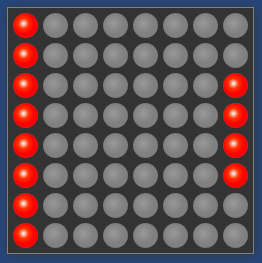
\includegraphics[width=0.7\linewidth, height=0.4\textheight]{screenshot003}
	\caption{}
	\label{fig:screenshot003}
\end{figure}


	Estas partes coinciden con las partes de la matriz menos usadas a la hora de escribir un numero.

	
	
  
\end{document}